\documentclass[a4paper,
fontsize=11pt,
%headings=small,
oneside,
numbers=noperiodatend,
parskip=half-,
bibliography=totoc,
final
]{scrartcl}

\usepackage{synttree}
\usepackage{graphicx}
\setkeys{Gin}{width=.9\textwidth} %default pics size

\graphicspath{{./plots/}}
\usepackage[english]{babel}
\usepackage[T1]{fontenc}
%\usepackage{amsmath}
\usepackage[utf8x]{inputenc}
\usepackage [hyphens]{url}
\usepackage{booktabs} 
\usepackage[left=2.4cm,right=2.4cm,top=2.3cm,bottom=2cm,headheight=25.60228pt,includeheadfoot]{geometry}
\usepackage{eurosym}
\usepackage{multirow}
\usepackage[english]{varioref}
\setcapindent{1em}
\renewcommand{\labelitemi}{--}
\usepackage{paralist}
\usepackage{pdfpages}
\usepackage{lscape}
\usepackage{float}
\usepackage{acronym}
\usepackage{eurosym}
\usepackage[babel]{csquotes}
\usepackage{longtable,lscape}
\usepackage{mathpazo}
\usepackage[flushmargin,ragged]{footmisc} % left align footnote

%%url brekas grrr
\expandafter\def\expandafter\UrlBreaks\expandafter{\UrlBreaks%  save the current one
  \do\a\do\b\do\c\do\d\do\e\do\f\do\g\do\h\do\i\do\j%
  \do\k\do\l\do\m\do\n\do\o\do\p\do\q\do\r\do\s\do\t%
  \do\u\do\v\do\w\do\x\do\y\do\z\do\A\do\B\do\C\do\D%
  \do\E\do\F\do\G\do\H\do\I\do\J\do\K\do\L\do\M\do\N%
  \do\O\do\P\do\Q\do\R\do\S\do\T\do\U\do\V\do\W\do\X%
  \do\Y\do\Z}%

\usepackage{listings}

\urlstyle{same}  % don't use monospace font for urls

\usepackage[fleqn]{amsmath}

%adjust fontsize for part

%% geometry
\clubpenalty = 10000 
\widowpenalty = 10000 
\displaywidowpenalty = 10000
%% tightlist

\providecommand{\tightlist}{%
  \setlength{\itemsep}{0pt}\setlength{\parskip}{0pt}}

\usepackage{sectsty}
\partfont{\large}

%Das BibTeX-Zeichen mit \BibTeX setzen:
\def\symbol#1{\char #1\relax}
\def\bsl{{\tt\symbol{'134}}}
\def\BibTeX{{\rm B\kern-.05em{\sc i\kern-.025em b}\kern-.08em
    T\kern-.1667em\lower.7ex\hbox{E}\kern-.125emX}}

\usepackage{fancyhdr}
\fancyhf{}
\pagestyle{fancyplain}
\fancyhead[R]{\thepage}

%meta

%meta

\fancyhead[L]{J. Schöpfel \& H. Prost \\ %author
LIBREAS. Library Ideas, 29 (2016). % journal, issue, volume.
\href{http://nbn-resolving.de/urn:nbn:de:kobv:11-100238193
}{urn:nbn:de:kobv:11-100238193}} % urn
\fancyhead[R]{\thepage} %page number
\fancyfoot[L] {\textit{Creative Commons BY 3.0}} %licence
\fancyfoot[R] {\textit{ISSN: 1860-7950}}

\title{\LARGE{Research data management in social sciences and humanities: A survey at the University of Lille (France)
}} %title %title
\author{Joachim Schöpfel \& Hélène Prost} %author

\setcounter{page}{}

\usepackage[colorlinks, linkcolor=black,citecolor=black, urlcolor=blue,
breaklinks= true]{hyperref}

\date{}
\begin{document}

\maketitle
\thispagestyle{fancyplain} 

%abstracts
\begin{abstract}
The paper presents results from a campus-wide survey at the University
of Lille (France) on research data management in social sciences and
humanities. The survey received 270 responses, equivalent to 15\% of the
whole sample of scientists, scholars, PhD students, administrative and
technical staff (research management, technical support services); all
disciplines were represented. The responses show a wide variety of
practice and usage. The results are discussed regarding job status and
disciplines and compared to other surveys. Four groups can be
distinguished, i.e.~pioneers (20-25\%), motivated (25-30\%), unaware
(30\%) and reluctant (5-10\%). Finally, the next steps to improve the
research data management on the campus are presented.


\end{abstract}

%body
\section*{Introduction}\label{introduction}

Research data management is a central part of the European Open Science
Agenda in the field of research and innovation. For the European
Commission (EC),

\enquote{\enquote{Open Science} is the transformation, opening up and
democratisation of science, research and innovation, with the objective
of making science more efficient, transparent and interdisciplinary, of
changing the interaction between science and society, and of enabling
broader societal impact and innovation} (Ramjoué 2015, p.169).

\enquote{Open research data} is one of the key components of the
emerging new ecosystem of standards and services, and the EC priorities
include \enquote{raising awareness regarding data management,
interoperability of infrastructure and datasets, and re-usability of
data} (\emph{ibid}.). In France, the Conference of University Presidents
put the issue of research data preservation and sharing at the top of
their priorities during their annual conference in 2015, the Ministry of
Higher Education and Research supports and promotes related actions, and
all major public research organizations such as the CNRS (\emph{Centre
national de la recherche scientifique)} contribute to the development of
data infrastructures and repositories.

The main issues and objectives are the same as in Germany or other
countries, i.e.~long-term preservation of scientific output and a global
policy of open data in order to increase transparency and stimulate
research, innovation and economic activity. There is a general consensus
about the complexity and the diversity of the field. Not only are
research data difficult to define but their handling and processing
largely depends on institutional and disciplinary practices and
behaviours; obviously, the term research data

\enquote{must always be viewed in relation to a particular subject
discipline (\ldots{}) all requirements for the management and long-term
availability of research data must be differentiated from each other in
regard to both general and discipline-specific aspects and solutions
(and) thus far, there is no general agreement on the definition of
digital curation, not only in Germany, but on international levels as
well} (Neuroth et al. 2013, p.11);

one size does not fit all. Also, organizational or national policies and
projects (top-down) require support and back-up from the scientific
communities and local structures (bottom-up) to meet the scientists'
needs with success.

\enquote{To support the step-by-step development of sound research data
management practices, you must first understand researchers' needs and
perspectives} (Ward et al. 2011, p.265). At Lille, we started in 2013 to
work in the field of research data management, in particular on the
social sciences and humanities campus (Lille 3) with 19,000 students,
580 PhD students, 850 academic and 600 technical staff, in order to
gather empirical evidence for the development of data literacy programs
and new library-based data services and to raise awareness among
scholars and PhD students. This research is conducted together with the
GERiiCO laboratory (information, communication and cultural studies),
the graduate school and the academic library, with the support of the
University's research department. The following study is work in
progress. We present the results of a campus-wide survey on data
practices and needs in 2015 and compare them with other studies,
including those from Humboldt-Universität zu Berlin (Simukovic et al.
2013, 2014). The complete results have already been published on our
institutional repository HAL-Lille 3 (Prost \& Schöpfel 2015). The
further reading section contains other papers on our research work.

\section*{Methodology}\label{methodology}

The campus-wide survey was conducted in April and May 2015 (five weeks).
The questionnaire contained 22 questions adapted from the survey from
Humboldt-Universität zu Berlin mentioned above, comprising six sections:
information about the respondent, data typology (sources and results),
preservation and backup behaviour, sharing behaviour, opinion and
motivation regarding data sharing and data repositories, data-related
needs. The questionnaire (in French) was communicated to the whole
research community on the social sciences and humanities campus (1,800
persons) in the form of an anonymous online version on a local
LimeSurvey server. The data analysis and interpretation was done between
June and August 2015, and the data were compared to other results from
Berlin (Simukovic et al. 2013, 2014), Strasbourg (Rege 2015, Rebouillat
2015), Iowa (Averkamp et al. 2014), LIBER (Reilly et al. 2011), the
European Commission (Kuipers \& van der Hoeven 2009, see also Herb 2015)
and Austria (Bauer et al. 2015).

\section*{Results}\label{results}

\paragraph{Response rate}\label{response-rate}

The survey received 270 responses, equivalent to 15\% of the whole
sample of scientists, scholars, PhD students, administrative and
technical staff (research management, technical support services). All
scientific departments and research laboratories are represented. Larger
and representative sub-samples are from psychology, history, education,
information and communication sciences.

Also, all professional groups took part in the survey. The largest group
of sub-samples are PhD students (n=73) and senior lecturers (n=69),
followed by professors (n=40), scientists (n=16) and other staff (n=13).
But the most representative group are professors (26\%), followed by
senior lecturers (17\%) and PhD students (13\%).

All respondents were asked to answer to the whole list of 22 questions
but no question was obligatory. Multiple answers were allowed for most
questions. As a result, no question received 100\% answers, and the
response rate per question varies between 12\% and 82\%.

\paragraph{Current research data
management}\label{current-research-data-management}

One part of the questions was about research data behaviour -- which
kind of data are used and produced, how they are stored, preserved,
safeguarded; and how they are shared with other researchers. The
responses show a wide variety of practice and usage.

\paragraph{Data sources}\label{data-sources}

The survey identified text documents as the most important data source,
followed by observations, interviews and survey data (figure 1).

\begin{figure}[htbp]
\centering
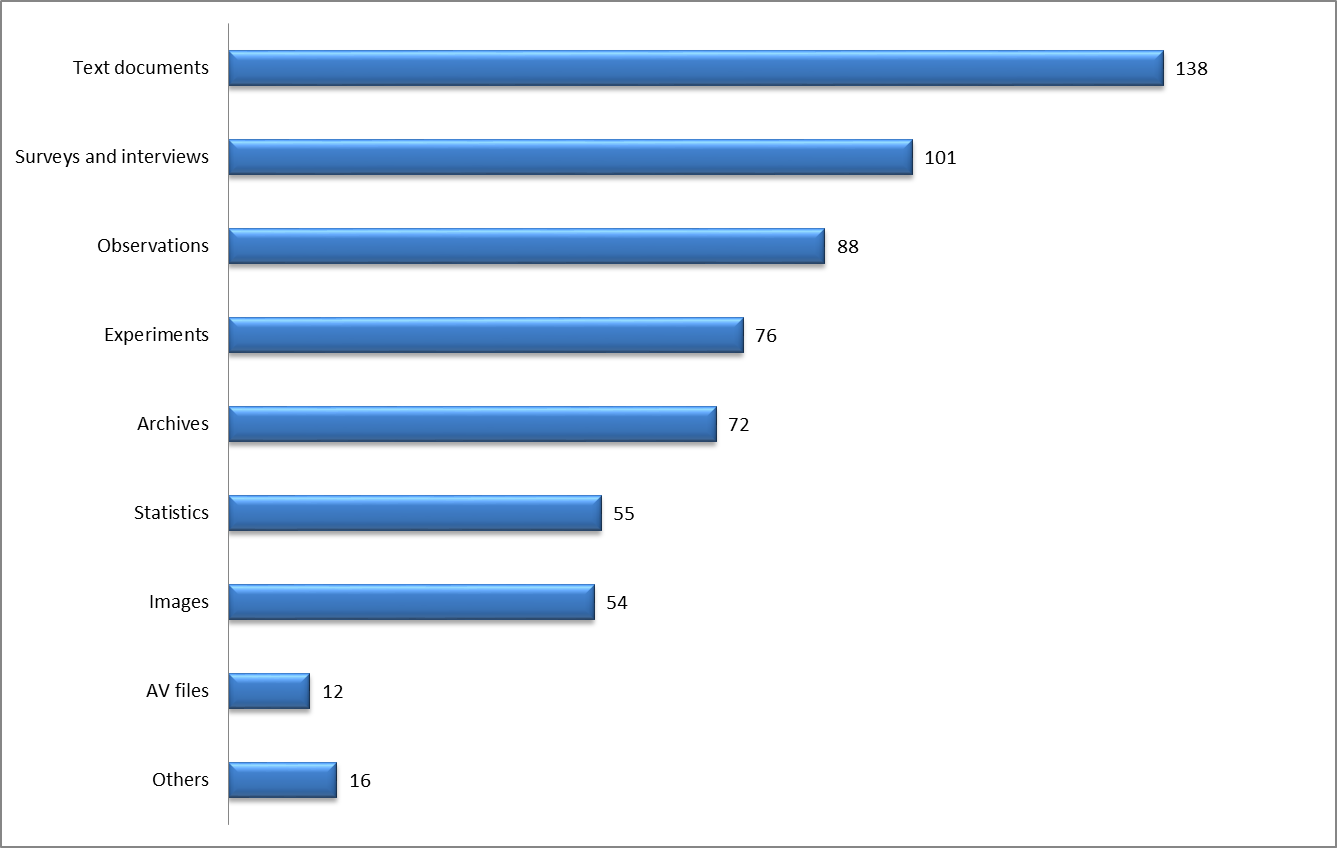
\includegraphics{figures/media/image1.png}
\caption{Research data sources (n=214)}
\end{figure}

Other, less important data sources are experiments, archival material,
statistics, images, and audio and video recordings, while log files or
simulations are missing, at least in our sample.

\paragraph{Data types}\label{data-types}

Figure 2 shows the research data produced by the respondents. Again,
text documents are the most important output type, followed by
spreadsheets, databases, multi-dimen\-sional visualisations and models.

\begin{figure}[htbp]
\centering
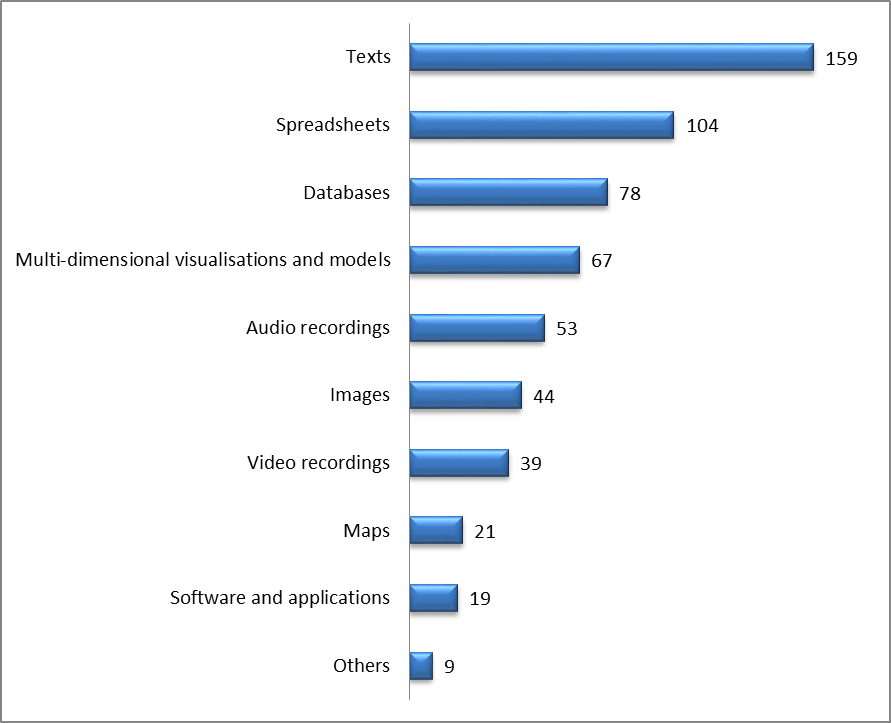
\includegraphics{figures/media/image2.png}
\caption{Research data types (n=211)}
\end{figure}

Other data types like audio and video recordings, images, maps or
software are less important.

\paragraph{Data storage}\label{data-storage}

Most of the respondents prefer local solutions for the storage of their
research data, either the hard disk of their private personal computer
(83\%), or their professional work-station (49\%) (figure 3).

\begin{figure}[htbp]
\centering
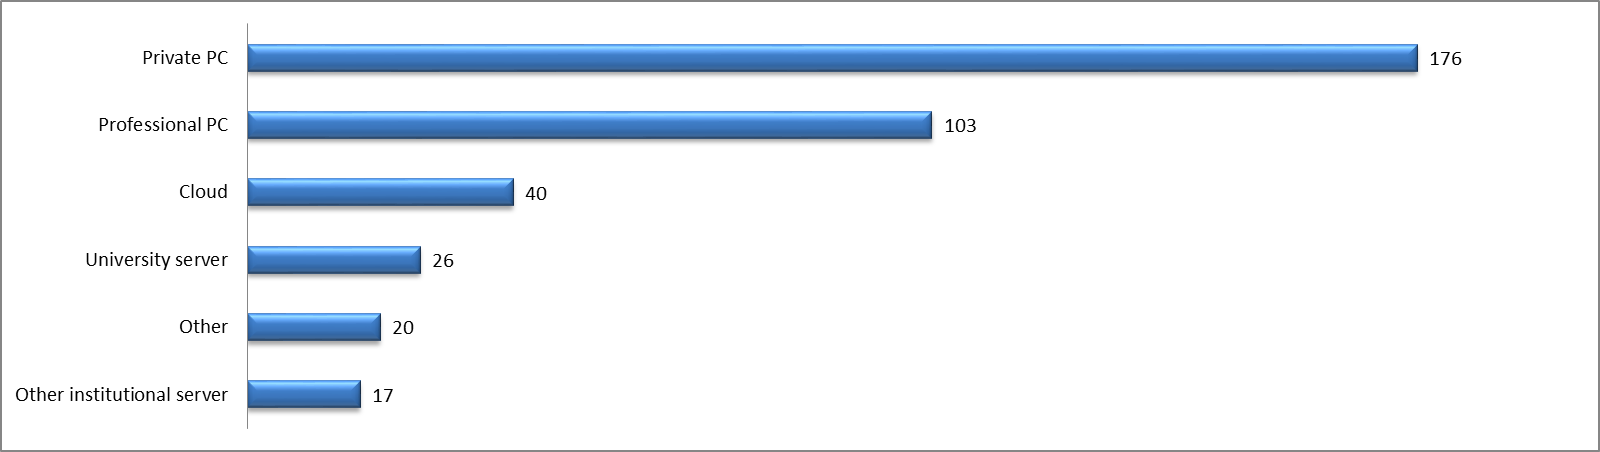
\includegraphics{figures/media/image3.png}
\caption{Storage places (n=212)}
\end{figure}

Only 12\% store their data on a campus-based server. 19\% conserve their
data in the cloud, on a distant server (gratis or not), and 8\% store
them on another institution's server, probably in collaborative,
multi-site research projects.

55\% say that they store their data in two or more different places,
which means usually on the personal (private) computer and on the
work-station on the campus. 76\% say that they also make use of other
devices, most often external hard drives (61\%) and USB flash drives
(46\%) while other devices such as CD or DVD are mentioned by few.

How much memory space do they occupy? 38\% of the respondents do not
know exactly. 51\% estimate their storage size at up to 100 gigabytes
while only 13 respondents (half of them are psychologists) mentioned 1
terabytes or more. While 28\% state that they back up the data on a
daily schedule, nearly as many (26\%) do it on an irregular basis,
\enquote{each time when needed} or \enquote{from time to time}. Nearly
all of them (97\%) say that they are the only people in charge of the
preservation of their research data and that there is no \enquote{data
officer} or at least another person specifically designated to perform
this task.

Taken together and as a whole, these responses appear to reflect a more
or less individual data behaviour, private rather than professional,
with available, often private (and cheap) devices but caring for
security and backup. We cannot say if the respondents already faced
serious problems with their research data (loss of data, security breach
etc.); probably they never have because they do not seem really
unsatisfied with this situation.

\paragraph{Data sharing}\label{data-sharing}

Most respondents (64\%) do not share their research data with colleagues
or other people (figure 4). Nobody, except themselves, have access to
their data files.

\begin{figure}[htbp]
\centering
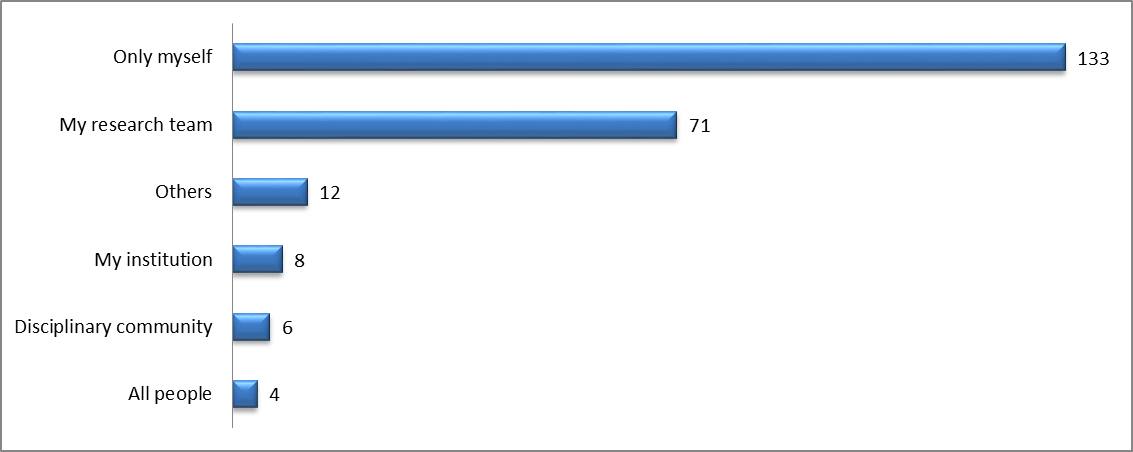
\includegraphics{figures/media/image4.png}
\caption{Access to research data (n=209)}
\end{figure}

Only 34\% share data with their colleagues and/or members of their
research team, and only 5\% share them with a wider audience, in an open
data approach \emph{stricto senso}.

Few replied to the question about the reuse of data produced by other
researchers (58\%), and even fewer (38\%, i.e.~22\% of the whole sample)
said that they had already downloaded this kind of scientific output and
8\% added that they will try in the future. Also, very few answered that
they were not interested or motivated to reuse other researchers' data.
One third (38\%) simply were (are) not aware of this opportunity and way
of doing science.

\paragraph{Needs}\label{needs}

Which kind of service and/or support or advice would they like to have?
The questionnaire proposed nine different types of data-related service,
from legal advice to technical infrastructure. Only 5\% of the
respondents state that they did not need any service. Most of the other
respondents indicated two or more needs (figure 5).

\begin{figure}[htbp]
\centering
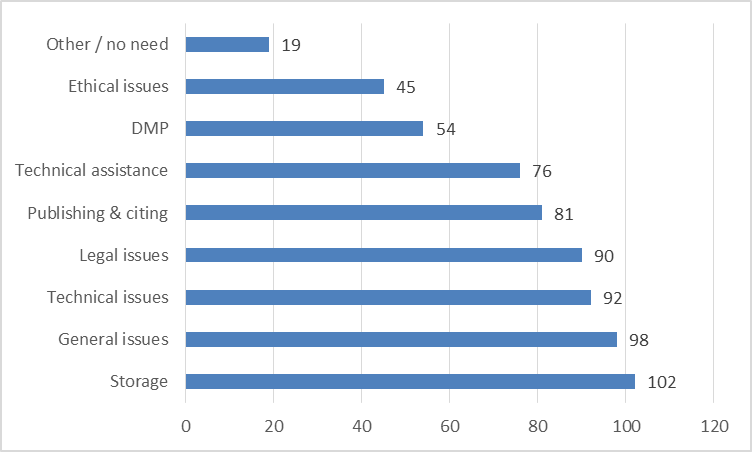
\includegraphics{figures/media/image5.png}
\caption{Support and services needed (n=188)}
\end{figure}

The survey does not really identify one or two priorities. The answers
rather reflect a set of needs, some more important (storage space,
general advice for data management), others a little bit less (technical
and legal issues, publishing and citing). One third mentioned ethical
issues and help for the preparation of data management plans (DMP).

\paragraph{Open access}\label{open-access}

We also tried to measure the colleagues' general willingness to deposit
and share their data. Are they motivated? Which kind of data would they
deposit? Would they publish their data along with articles? Which data
repository would they prefer?

About 40\% of the respondents express a positive opinion about data
sharing. Either they have already deposited their data in a repository
(16\%) or they intend to do so in the future (25\%). 30\% admit that
they were not aware of this possibility (figure 6).

\begin{figure}[htbp]
\centering
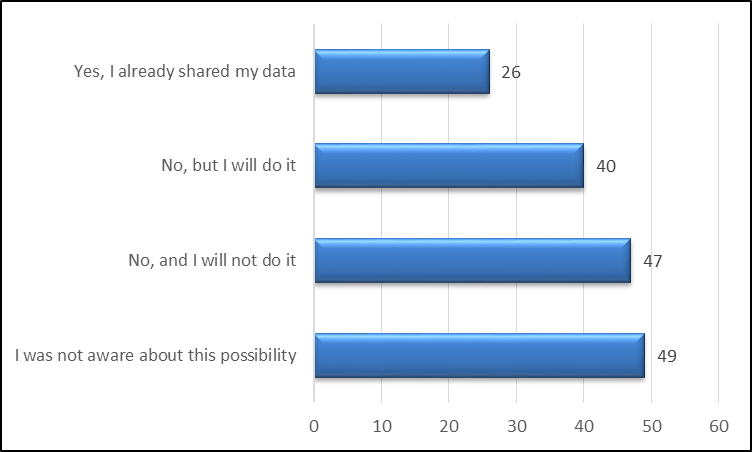
\includegraphics{figures/media/image6.png}
\caption{Deposit of research data in a data repository (n=162)}
\end{figure}

Another third (29\%) clearly say that they never deposited their
research data in the past and that they have no intention of doing so in
the future. A deposit in a data repository is no option for five
reasons: sensitive and confidential data, risk of plagiarism, workload,
data illegibility (\enquote{nobody would understand my raw data}) and
intellectual property (\enquote{these are MY data}).

This rejection of data sharing significantly decreases when it comes to
the question of publishing data along with an article, i.e.~when data
sharing is incentive or obligatory (figure 7). Here, only 7\% declare
that they never shared their data in the past and that they will not
share them in the future.

\begin{figure}[htbp]
\centering
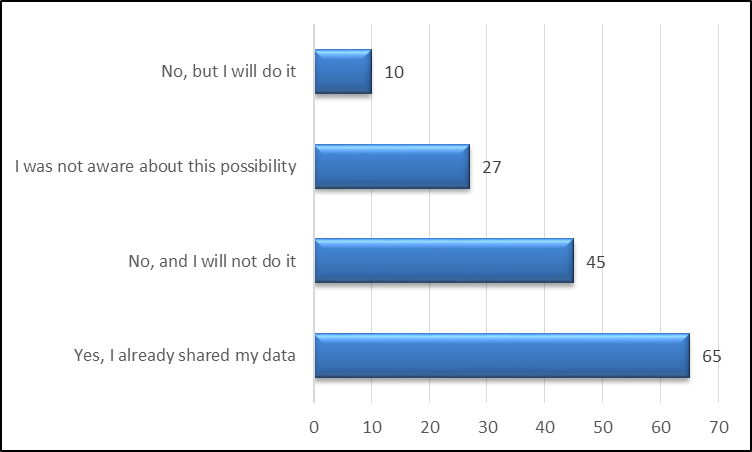
\includegraphics{figures/media/image7.png}
\caption{Data publishing (n=147)}
\end{figure}

44\% of the respondents state that they have already published data
together with an article, and 31\% announce that they intend to do so in
the future while 18\% admit that they simply did not know about this
possibility.

We also asked when and which kind of data they would share. Again, only
12\% clearly state that they will not deposit or share their research
results in this way (figure 8).

\begin{figure}[htbp]
\centering
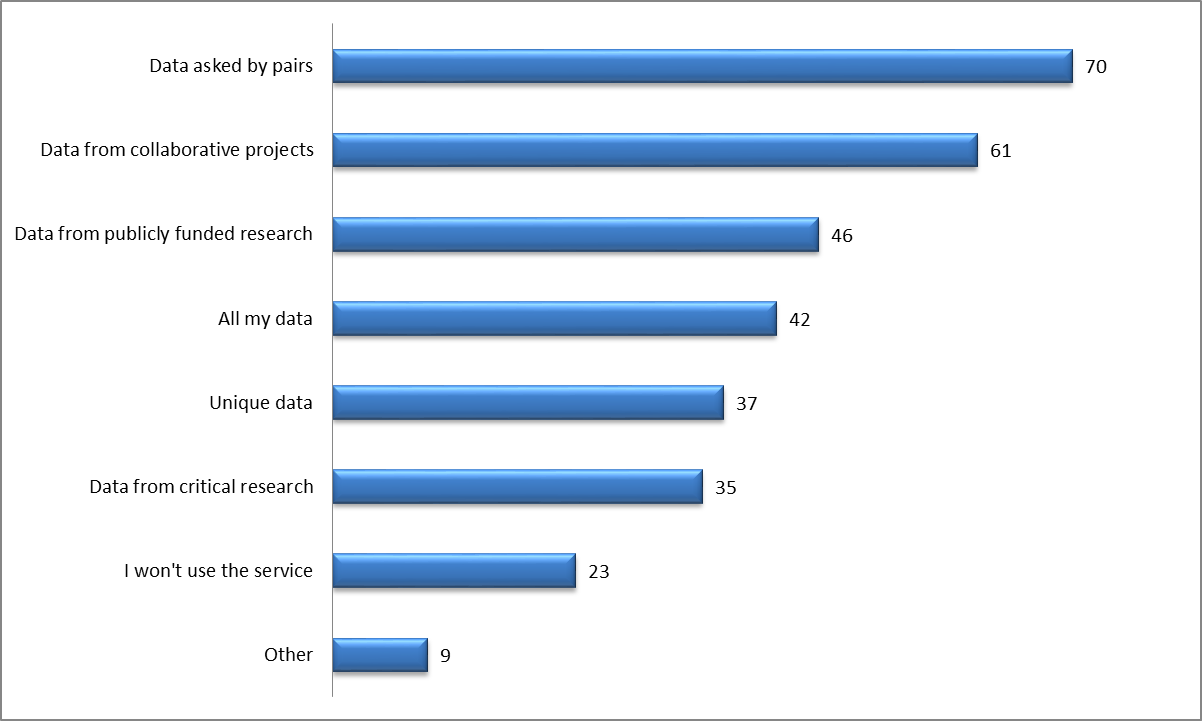
\includegraphics{figures/media/image8.png}
\caption{Data deposit (n=187)}
\end{figure}

37\% underline that they would share those data asked for by their peers
while others say that they would deposit data produced in collaborative
research projects (33\%) or with public funding (25\%). The last
question was about the kind of repository they would prefer for the
deposit and sharing of their research data (figure 9). Even without a
clear preference (many respondents mark more than one answer), we can
identify a ranking of preferred options.

\begin{figure}[htbp]
\centering
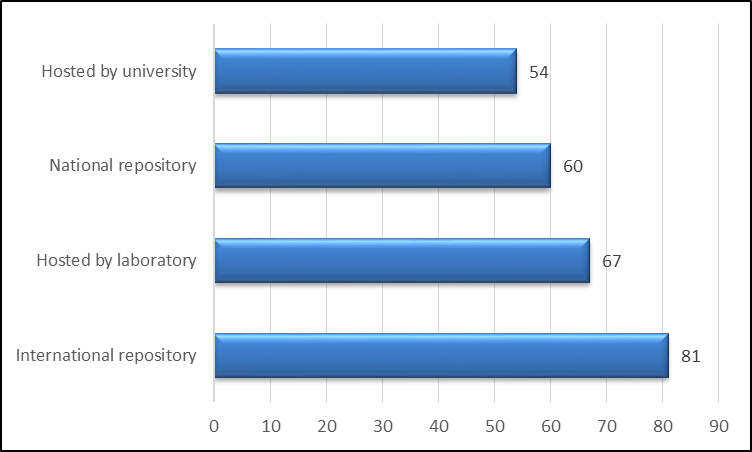
\includegraphics{figures/media/image9.png}
\caption{Preferred data repository (n=173)}
\end{figure}

International data repositories (47\%) are at the top of the ranking,
followed by local servers hosted by the laboratory, i.e.~the research
institute (39\%). National (35\%) or campus-wide platforms (31\%) are
less preferred. In other words, this sample is more interested in impact
and visibility (international repository) and disciplinary specificity
(laboratory) than in a multidisciplinary, national or institutional
solution. Yet, no alternative is really rejected, and the differences do
not seem to be very significant.

\section*{Discussion}\label{discussion}

The response rate of this study -- 15\% - is globally satisfying,
compared with other surveys in the same field where the rate is
partially unknown (Tenopir et al. 2011 and 2015, Averkamp et al. 2014)
or varying from 7\% (Rege 2015) and 9\% (Bauer et al. 2015) to 24\%
(Simukovic et al. 2013 and 2014). We received more answers from PhD
students (33\%) than in other surveys\footnote{Berlin 23\% (Simukovic et
  al. 2013), Strasbourg 10\% (Rege 2015), international NSF survey
  13.5\% (Tenopir et al. 2011)}. However, the rather small sample of 270
respondents should induce caution, especially when comparing
sub-samples. Therefore, the following discussion will report tendencies
rather than representative and reliable results.

Another reason for a prudent interpretation is the response rate per
question. While questions about data management received an average
response rate of 78\%, the response rate for questions about data
sharing fell to 49\%. This low response rate may reflect a lack in a mix
of experience, knowledge, motivation and awareness. But in all cases, it
reduces still further the reliability of the replies.

As a whole, our sample does not confirm the 60-40 rule from the European
PARSE.insight project which states that \enquote{60\% like to get data
from others but 40\% have problems to give their own} (Reilly et al.
2011, p.12). In the Lille survey, only 46\% (and not 60\%) like to get
data from others, and only 29\% have problems giving their own away,
with 30\% others who have not made up their minds so far, for lack of
information and/or awareness. On the whole, the scientists, scholars and
PhD students seem rather pragmatic and realistic on a social sciences,
humanities and arts campus with an extensive education program and a
rather low budget for research.

\paragraph{Status and discipline}\label{status-and-discipline}

To most of the survey questions, the professors, senior lecturers and
PhD students replied in a consistent and comparable way, without any
significant differences. The survey confirms that PhD students have less
experience with research data management and sharing and are less aware
of data-related aspects. But they also show a higher motivation to
deposit and share their data in the future (63\%) than professors and
senior lecturers who seem more reluctant to deposit (45\%). Professors
are also twice more reluctant (28\%) than PhD students (13\%) to reuse
the research data produced by other scientists. But all agree that they
would prefer international data repositories to local solutions.

Our survey also reveals some differences between scientific communities
(disciplines) on the campus. For instance, scholars in psychology and
education seem less aware of data management and sharing than those in
history, information sciences and modern languages and literature. Yet,
statistically speaking, these are tendencies rather than significant
differences, and as a whole, our sample shows a rather homogeneous
community of scholars and scientists in social sciences and humanities,
at least regarding research data management. Disciplinary differences
exist but they should not be over-interpreted.

\paragraph{Clusters}\label{clusters}

On the whole, we can distinguish four groups in our sample but they are
not related to status or discipline. According to the answers on data
management practice and motivation to share research data, we can
identify four \enquote{clusters} of scholars and scientists (in
brackets, the estimated part of the whole sample):

\begin{itemize}
\item
  The pioneers (20-25\%): These respondents have more experience with
  data management and deposit and are more inclined to future data
  sharing than their colleagues.
\item
  The motivated (25-30\%): A second group of scholars and scientists
  with less or no experience are nevertheless highly motivated to engage
  in data sharing in the future.
\item
  The unaware (30\%): About one third of the sample admit that they are
  not really aware of research data management, of the opportunities for
  sharing their results with others or of the possibility to reuse the
  data of other scientists.
\item
  The reluctant (5-10\%): A small group did not deposit or share their
  data up to now and state that they will not do so in the future
  either.
\end{itemize}

Of course, the boundaries between these clusters are not always evident,
in particular between the \enquote{pioneers} and the
\enquote{motivated}. Also, because of the small size of the sub-samples,
we did not try to characterize these clusters with regards to job status
and discipline. More important for us is (1) the empirical evidence of
different groups, a fact that calls for a differential approach on the
campus, and (2) the relative part of each cluster, in particular the
relatively small size of the \enquote{reluctant group}.

\paragraph{Comparison with other
surveys}\label{comparison-with-other-surveys}

Compared to the results of other surveys\footnote{Berlin n=499
  (Simukovic et al. 2013, 2014)~; Strasbourg n=644 (Rege 2015,
  Rebouillat 2015)~; LIBER n=1840 (Reilly et al. 2011, Kuipers \& van
  der Hoeven 2009, cf.~also Herb 2015)~; Iowa n=784 (Averkamp et al.
  2014)~; Austria n=3,026 (Bauer et al. 2015)~; international NSF survey
  n=1,315 (Tenopir et al. 2011) and follow-up n=1,015 (Tenopir et al.
  2015)}, we can highlight three aspects:

\begin{itemize}
\item
  Data management: less experience and a more personal (private)
  practice, especially regarding the way data are stored and backed up.
  At the University of Iowa, 69\% store their data on their private
  computers but 72\% (also) on a shared drive or institutional server.
  Austrian scientists mainly use their work computers (71\%) and
  external storage devices (64\%), while only 54\% store the data on
  their private computers.
\item
  Data sharing: a lower percentage of respondents already share data
  (34\%), compared to the Berlin (50\%), LIBER (58\%) or NSF follow-up
  (75\%) surveys. The Austrian scientists reported that they grant
  access to their data on request (57\%) or to members of their own
  institution (53\%). However, only 28\% made their data available to
  the scientific community and only 10\% to a wider public. These
  figures are more in line with our own results, such as the first NSF
  survey where only 36\% scientists stated that they made their data
  easily accessible (Tenopir et al. 2011).
\item
  Attitude towards data sharing: less favourable (40\%) than the Berlin
  survey (60\%), yet not more reluctant (12\% compared to 15\% in Berlin
  or 10\% in Austria). The first NSF survey revealed that nearly half of
  the respondents would not share their data with others (46\%) but the
  follow-up study shows that this percentage is decreasing.
\end{itemize}

One reason for these differences may be the fact that the Lille 3 survey
puts the focus on social sciences and humanities. Other aspects are
consistent with the cited surveys, such as the mainly personal
responsibility for data management (93\% \enquote{myself} in the Austria
survey) and the preference for international and decentralized
institutional data repositories (47\% and 37\%, Austria survey). The NSF
follow-up study confirmed that scientists in psychology and education
are in average less interested in data sharing, probably because of the
often non-anonymous character of their results.

\section*{Conclusion}\label{conclusion}

The Lille survey provides a photography of a dynamic situation. Tenopir
et al. (2015) described this situation as a \enquote{complex shift, with
varying cultures among scientists that dictate the norms surrounding
data sharing and reuse (and) still perceived risks and barriers that may
be slowing the data sharing movement}. However, our study also showed
that the continued barriers affect only a small part of the scientists,
scholars and PhD students and that most of them are not opposed to data
sharing but may need more information about conditions and
opportunities.

The survey results helped us to improve the information about data
management, deposit and sharing and to launch a training program for PhD
students, as part of their doctoral education, as we are convinced that
\enquote{the best possible point at which to intervene with guidance and
training is very early on in a researcher's career} (Ward et al. 2011,
p.268). The survey itself also raised awareness on the issue of data
management and data sharing and on the data policy on the Lille 3
campus\footnote{For instance, we published a white paper on data in
  dissertations (Chaudiron et al. 2015), we organize an international
  conference on electronic dissertations and research data (ETD2016) and
  we develop our library based service on research data, also in
  collaboration with the UK JISC.}. The next step will be the project of
a Lille data repository, either for all disciplines or limited to social
sciences and humanities, in the framework of the French data
infrastructure in digital humanities\footnote{\url{http://www.huma-num.fr/}}.
All these actions (figure 10) are coordinated and supported by the
academic library, the graduate school in social sciences and humanities,
the GERiiCO research laboratory, the University's research management
and the European Institute for Social Sciences and Humanities\footnote{\url{http://www.meshs.fr/}}
at Lille.

\begin{figure}[htbp]
\centering
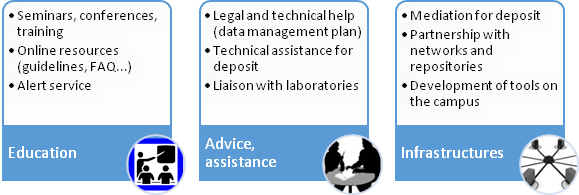
\includegraphics{figures/media/image10.png}
\caption{Research data support services}
\end{figure}

The academic library plays a central part in particular in education,
advice and assistance. The library will also be partner to a series of
in-depth interviews with a smaller sample of scientists (n=30-50) in
order to learn more about data behaviour, best practices and
data-related needs. And the academic librarians' contribution is
expected and necessary also for the development of infrastructures and
tools.

\section*{Acknowledgments}\label{acknowledgments}

The study was supported by the Department of International Relations of
the University of Lille 3 and the European Institute for Social Sciences
and Humanities at Lille. We would like to thank all colleagues who
contributed to the success of the survey, in particular Peter
Schirmbacher, Maxi Kindling and Elena Simukovic (Berlin), Isabelle
Westeel, Cécile Malleret and Stéphane Chaudiron (Lille).

\section*{References}\label{references}

Averkamp, S., Gu, X., Rogers, B., 2014. \emph{Data management at the
University of Iowa: A university libraries report on campus research
data needs}. University of Iowa. \url{http://ir.uiowa.edu/lib_pubs/153/}

Bauer, B., Ferus, A., Gorraiz, J., Gumpenberger, C., Gründhammer, V.,
Maly, N., Mühlegger, J. M., Preza, J. L., Sánchez Solís, B., Schmidt,
N., Steineder, C., 2015. \emph{Researchers and their data. Results of an
Austrian survey - report 2015}. e-infrastructures austria, Vienna.
\url{http://e-infrastructures.at/das-projekt/deliverables/}

Chaudiron, S., Maignant, C., Schöpfel, J., Westeel, I., 2015.
\emph{Livre blanc sur les données de la recherche dans les thèses de
doctorat}. Université de Lille 3, Villeneuve d'Ascq.
\url{http://hal.univ-lille3.fr/hal-01192930}

Herb, U., 2015. \emph{Open Science in der Soziologie. Eine
interdisziplinäre Bestandsaufnahme zur offenen Wissenschaft und eine
Untersuchung ihrer Verbreitung in der Soziologie}. vwh Verlag Werner
Hülsbusch, Glückstadt.

Kuipers, T., van der Hoeven, J., 2009. \emph{Insight into digital
preservation of research output in Europe. Survey report.} PARSE
insight, European Commission, Brussels.
\url{http://www.parse-insight.eu/downloads/PARSE-Insight_D3-4_SurveyReport_final_hq.pdf}

Neuroth, H., Strathmann, S., Oßwald, A., Ludwig, J. (Eds.), 2013.
\emph{Digital curation of research data. Experiences of a baseline study
in Germany}. vwh Verlag Werner Hülsbusch, Glückstadt.
\url{http://www.nestor.sub.uni-goettingen.de/bestandsaufnahme/Digital_Curation.pdf}

Prost, H., Schöpfel, J., 2015. \emph{Les données de la recherche en SHS.
Une enquête à l'Université de Lille 3.} Rapport final. Université de
Lille 3, Villeneuve d'Ascq.
\url{http://hal.univ-lille3.fr/hal-01198379v1}

Ramjoué, C., 2015. Towards Open Science: The vision of the European
Commission. \emph{Information Services \& Use 35} (3), 167-170.
\url{http://doi.org/10.3233/isu-150777}

Rebouillat, V., 2015. \emph{Archives ouvertes de la connaissance :
Valoriser et diffuser les données de recherche}. Master's thesis,
ENSSIB, Villeurbanne.
\url{http://cataloguebib.enssib.fr/cgi-bin/koha/opac-detail.pl?biblionumber=1903}

Rege, A., 2015. Retour sur l'enquête sur les pratiques de publication
scientifique et de production de données de la recherche. In:
\emph{Université de Strasbourg, Projet AOC}, COPIL 27 mars 2015.

Reilly, S., Schallier, W., Schrimpf, S., Smit, E., Wilkinson, M., 2011.
\emph{Report on integration of data and publications}. ODE Opportunities
for Data Exchange, The Hague.
\url{http://www.stm-assoc.org/2011_12_5_ODE_Report_On_Integration_of_Data_and_Publications.pdf}

Simukovic, E., Kindling, M., Schirmbacher, P., 2013. \emph{Umfrage zum
Umgang mit digitalen Forschungsdaten an der Humboldt-Universität zu
Berlin.} Report, Humboldt-Universität zu Berlin, Zentraleinrichtung
Computer- und Medienservice (Rechenzentrum), Berlin.
\url{http://edoc.hu-berlin.de/docviews/abstract.php?id=40341}

Simukovic, E., Kindling, M., Schirmbacher, P., 2014. Unveiling research
data stocks: A case of Humboldt-Universität zu Berlin. In:
\emph{iConference}, 4-7 March 2014, Berlin. pp.~742-748.
\url{https://www.ideals.illinois.edu/handle/2142/47259}

Tenopir, C., Allard, S., Douglass, K., Aydinoglu, A. U., Wu, L., Read,
E., Manoff, M., Frame, M., 2011. Data sharing by scientists: Practices
and perceptions. \emph{PLoS ONE} 6 (6), e21101+.
\url{http://doi.org/10.1371/journal.pone.0021101}

Tenopir, C., Dalton, E. D., Allard, S., Frame, M., Pjesivac, I., Birch,
B., Pollock, D., Dorsett, K., 2015. Changes in data sharing and data
reuse practices and perceptions among scientists worldwide. \emph{PLoS
ONE} 10 (8), e0134826+.
\url{http://doi.org/10.1371/journal.pone.0134826}

Ward, C., Freiman, L., Jones, S., Molloy, L., Snow, K., Jul. 2011.
Making sense: Talking data management with researchers.
\emph{International Journal of Digital Curation} 6~(2),
265-273.~\url{http://doi.org/10.2218/ijdc.v6i2.202}

\section*{Further readings}\label{further-readings}

Chaudiron, S., Maignant, C., Schöpfel, J., Westeel, I., 2015.
\emph{Livre blanc sur les données de la recherche dans les thèses de
doctorat.} Université de Lille 3, Villeneuve d'Ascq.
\url{http://hal.univ-lille3.fr/hal-01192930}

Prost, H., Malleret, C., Schöpfel, J., 2015. Hidden treasures. Opening
data in PhD dissertations in social sciences and humanities.
\emph{Journal of Librarianship and Scholarly Communication} 3 (2),
eP1230+. \url{http://doi.org/10.7710/2162-3309.1230}

Schöpfel, J., Chaudiron, S., Jacquemin, B., Prost, H., Severo, M.,
Thiault, F., 2014. Open access to research data in electronic theses and
dissertations: An overview. \emph{Library Hi Tech} 32 (4), 612-627.
\url{http://doi.org/10.1108/LHT-06-2014-0058}

Schöpfel, J., Prost, H., Malleret, C., 2015a. Making data in PhD
dissertations reusable for research. In: \emph{8th Conference on Grey
Literature and Repositories}, National Library of Technology (NTK), 21
October 2015, Prague, Czech Republic.
\url{http://hal.univ-lille3.fr/hal-01248979/document}

Schöpfel, J., Juznic, P., Prost, H., Malleret, C., Cesarek, A.,
Koler-Povh, T., 2015b. Dissertations and data (keynote address). In:
\emph{GL17 International Conference on Grey Literature}, 1-2 December
2015, Amsterdam. \url{http://hal.univ-lille3.fr/hal-01285304}

%autor
\begin{center}\rule{0.5\linewidth}{\linethickness}\end{center}

\textbf{Joachim Schöpfel} is Lecturer of Library and Information
Sciences at the University of Lille 3 (France), Director of the French
Digitization Centre for PhD theses (ANRT) and member of the GERiiCO
research laboratory. He was Manager of the INIST (CNRS) scientific
library from 1999 to 2008. He teaches Library Marketing, Auditing,
Intellectual Property and Information Science. His research interests
are scientific information and communication, particularly open access,
research data and grey literature.

\textbf{Hélène Prost} is an information professional at the Institute of
Scientific and Technical Information (CNRS) and associate member of the
GERiiCO research laboratory (University of Lille 3). She is interested
in empirical library and information sciences and statistical data
analysis. She participates in research projects on the evaluation of
collections, document delivery, usage analysis, grey fliterature and
open access, and she is the author of several publications.

\end{document}